% A LaTeX template for MSc Thesis submissions to 
% Politecnico di Milano (PoliMi) - School of Industrial and Information Engineering
%
% S. Bonetti, A. Gruttadauria, G. Mescolini, A. Zingaro
% e-mail: template-tesi-ingind@polimi.it
%
% Last Revision: October 2021
%
% Copyright 2021 Politecnico di Milano, Italy. NC-BY

\documentclass{Configuration_Files/PoliMi3i_thesis}
%------------------------------------------------------------------------------
%	REQUIRED PACKAGES AND  CONFIGURATIONS
%------------------------------------------------------------------------------

% CONFIGURATIONS
\usepackage{rotating, caption}
\usepackage{pdflscape}
\usepackage{pdfpages}
\usepackage{minted}
\usepackage{comment}
\usepackage{listings}
\usepackage{parskip} % For paragraph layout
\usepackage{setspace} % For using single or double spacing
\usepackage{emptypage} % To insert empty pages
\usepackage{multicol} % To write in multiple columns (executive summary)
\setlength\columnsep{15pt} % Column separation in executive summary
\setlength\parindent{0pt} % Indentation
\raggedbottom  

% PACKAGES FOR TITLES
\usepackage{titlesec}
% \titlespacing{\section}{left spacing}{before spacing}{after spacing}
\titlespacing{\section}{0pt}{3.3ex}{2ex}
\titlespacing{\subsection}{0pt}{3.3ex}{1.65ex}
\titlespacing{\subsubsection}{0pt}{3.3ex}{1ex}
\usepackage{color}

% PACKAGES FOR LANGUAGE AND FONT
\usepackage[english]{babel} % The document is in English  
\usepackage[utf8x]{inputenc} % UTF8 encoding
\usepackage[T1]{fontenc} % Font encoding
\usepackage[11pt]{moresize} % Big fonts

% PACKAGES FOR IMAGES
\usepackage{graphicx}
\usepackage{transparent} % Enables transparent images
\usepackage{eso-pic} % For the background picture on the title page
\usepackage{subfig} % Numbered and caption subfigures using \subfloat.
\usepackage{tikz} % A package for high-quality hand-made figures.
\usetikzlibrary{}
\graphicspath{{./Images/}} % Directory of the images
\usepackage{caption} % Coloured captions
\usepackage{xcolor} % Coloured captions
\usepackage{amsthm,thmtools,xcolor} % Coloured "Theorem"
\usepackage{float}

% STANDARD MATH PACKAGES
\usepackage{amsmath}
\usepackage{amsthm}
\usepackage{amssymb}
\usepackage{amsfonts}
\usepackage{bm}
\usepackage[overload]{empheq} % For braced-style systems of equations.
\usepackage{fix-cm} % To override original LaTeX restrictions on sizes

% PACKAGES FOR TABLES
\usepackage{tabularx}
\usepackage{longtable} % Tables that can span several pages
\usepackage{colortbl}

% PACKAGES FOR ALGORITHMS (PSEUDO-CODE)
\usepackage{algorithm}
\usepackage{algorithmic}


% PACKAGES FOR REFERENCES & BIBLIOGRAPHY
%\usepackage[colorlinks=true,linkcolor=black,anchorcolor=black,citecolor=black,filecolor=black,menucolor=black,runcolor=black,urlcolor=black]{hyperref} % Adds clickable links at references
%\usepackage{cleveref}
%\usepackage[square, numbers, sort&compress]{natbib} % Square brackets, citing references with numbers, citations sorted by appearance in the text and compressed
%\bibliographystyle{siam} % You may use a different style adapted to your field

% PACKAGES FOR REFERENCES & BIBLIOGRAPHY
\usepackage[colorlinks=true,linkcolor=black,anchorcolor=black,citecolor=black,filecolor=black,menucolor=black,runcolor=black,urlcolor=black]{hyperref} % Adds clickable links at references
\usepackage{cleveref}
\usepackage[square, numbers, sort&compress]{natbib} % Square brackets, citing references with numbers, citations sorted by appearance in the text and compressed
\bibliographystyle{abbrvnat} % You may use a different style adapted to your field


% OTHER PACKAGES
\usepackage{pdfpages} % To include a pdf file
\usepackage{afterpage}
\usepackage{lipsum} % DUMMY PACKAGE
\usepackage{fancyhdr} % For the headers
\fancyhf{}
\usepackage{eurosym}

% Input of configuration file. Do not change config.tex file unless you really know what you are doing. 
% Define blue color typical of polimi
\definecolor{bluepoli}{cmyk}{0.4,0.1,0,0.4}

% Custom theorem environments
\declaretheoremstyle[
  headfont=\color{bluepoli}\normalfont\bfseries,
  bodyfont=\color{black}\normalfont\itshape,
]{colored}

% Set-up caption colors
\captionsetup[figure]{labelfont={color=bluepoli}} % Set colour of the captions
\captionsetup[table]{labelfont={color=bluepoli}} % Set colour of the captions
%\captionsetup[algorithm]{labelfont={color=bluepoli}} % Set colour of the captions

\theoremstyle{colored}
\newtheorem{theorem}{Theorem}[chapter]
\newtheorem{proposition}{Proposition}[chapter]

% Enhances the features of the standard "table" and "tabular" environments.
\newcommand\T{\rule{0pt}{2.6ex}}
\newcommand\B{\rule[-1.2ex]{0pt}{0pt}}

% Pseudo-code algorithm descriptions.
%\newcounter{algsubstate}
%\renewcommand{\thealgsubstate}{\alph{algsubstate}}
%\newenvironment{algsubstates}
 % {\setcounter{algsubstate}{0}%
  % \renewcommand{\STATE}{%
   %  \stepcounter{algsubstate}%
    % \Statex {\small\thealgsubstate:}\space}}
  %{}

% New font size
\newcommand\numfontsize{\@setfontsize\Huge{200}{60}}

% Title format: chapter
\titleformat{\chapter}[hang]{
\fontsize{50}{20}\selectfont\bfseries\filright}{\textcolor{bluepoli} \thechapter\hsp\hspace{2mm}\textcolor{bluepoli}{|   }\hsp}{0pt}{\huge\bfseries \textcolor{bluepoli}
}

% Title format: section
\titleformat{\section}
{\color{bluepoli}\normalfont\Large\bfseries}
{\color{bluepoli}\thesection.}{1em}{}

% Title format: subsection
\titleformat{\subsection}
{\color{bluepoli}\normalfont\large\bfseries}
{\color{bluepoli}\thesubsection.}{1em}{}

% Title format: subsubsection
\titleformat{\subsubsection}
{\color{bluepoli}\normalfont\large\bfseries}
{\color{bluepoli}\thesubsubsection.}{1em}{}

% Shortening for setting no horizontal-spacing
\newcommand{\hsp}{\hspace{0pt}}

\makeatletter
% Renewcommand: cleardoublepage including the background pic
\renewcommand*\cleardoublepage{%
  \clearpage\if@twoside\ifodd\c@page\else
  \null
  \AddToShipoutPicture*{\BackgroundPic}
  \thispagestyle{empty}%
  \newpage
  \if@twocolumn\hbox{}\newpage\fi\fi\fi}
\makeatother

%For correctly numbering algorithms
%\numberwithin{algorithm}{chapter}

%----------------------------------------------------------------------------
%	NEW COMMANDS DEFINED
%----------------------------------------------------------------------------

% EXAMPLES OF NEW COMMANDS
\newcommand{\bea}{\begin{eqnarray}} % Shortcut for equation arrays
\newcommand{\eea}{\end{eqnarray}}
\newcommand{\e}[1]{\times 10^{#1}}  % Powers of 10 notation

%----------------------------------------------------------------------------
%	ADD YOUR PACKAGES (be careful of package interaction)
%----------------------------------------------------------------------------
%\usepackage{pgfplots}
\usepackage{lscape}
\usepackage{rotating}
\usepackage{lipsum}


%----------------------------------------------------------------------------
%	ADD YOUR DEFINITIONS AND COMMANDS (be careful of existing commands)
%----------------------------------------------------------------------------
\newsavebox{\mybox}
%----------------------------------------------------------------------------
%	BEGIN OF YOUR DOCUMENT
%----------------------------------------------------------------------------




\begin{document}


\fancypagestyle{plain}{%
\fancyhf{} % Clear all header and footer fields
\fancyhead[RO,RE]{\thepage} %RO=right odd, RE=right even
\renewcommand{\headrulewidth}{0pt}
\renewcommand{\footrulewidth}{0pt}}

%----------------------------------------------------------------------------
%	TITLE PAGE
%----------------------------------------------------------------------------

\pagestyle{empty} % No page numbers
\frontmatter % Use roman page numbering style (i, ii, iii, iv...) for the preamble pages

\puttitle{
	title=Controlling management systems applied to LPT Italian companies, % Title of the thesis
	name= \\ 
	      \vspace{0.2 cm}\\
	      Chiara Beretta \hspace{2,2 cm} 10615536 \\ 
          \vspace{0.01 cm}  \\   
          Seyed Hesam Babaei \hspace{0,99 cm} 10780315 \\ 
          \vspace{0.01 cm}\\ 
          Luca Cattaneo \hspace{2,2 cm} 10521219 \\ 
          \vspace{0.01 cm}\\          
          Pietro Mariano \hspace{2,1 cm} 10529938 \\
          \vspace{0.01 cm}\\
          Fabio Vitiello \hspace{2,5 cm} 10529938, % Author Name and Surname
	course= MOBILITY: INFRASTRUCTURES AND SERVICES , % Study Programme (in Italian)
	academicyear={2021-2022},  % Academic Year
} % These info will be put into your Title page 

%----------------------------------------------------------------------------
%	PREAMBLE PAGES: ABSTRACT (inglese e italiano), EXECUTIVE SUMMARY
%----------------------------------------------------------------------------
\startpreamble
\setcounter{page}{1} % Set page counter to 1

% ABSTRACT IN ENGLISH

\include{Chapters/00_Abstract}

%----------------------------------------------------------------------------
%	LIST OF CONTENTS/FIGURES/TABLES/SYMBOLS
%----------------------------------------------------------------------------

% TABLE OF CONTENTS
\thispagestyle{empty}
\tableofcontents % Table of contents 
\thispagestyle{empty}
\cleardoublepage

%-------------------------------------------------------------------------
%	THESIS MAIN TEXT
%-------------------------------------------------------------------------
% In the main text of your thesis you can write the chapters in two different ways:
%
%(1) As presented in this template you can write:
%    \chapter{Title of the chapter}
%    *body of the chapter*
%
%(2) You can write your chapter in a separated .tex file and then include it in the main file with the following command:
%    \chapter{Title of the chapter}
%    \input{chapter_file.tex}
%
% Especially for long thesis, we recommend you the second option.

%\addtocontents{toc}{\vspace{2em}} % Add a gap in the Contents, for aesthetics
\mainmatter % Begin numeric (1,2,3...) page numbering
% --------------------------------------------------------------------------
% NUMBERED CHAPTERS % Regular chapters following
% --------------------------------------------------------------------------
\chapter{Introduction}




















\chapter{State of the Art}

\paragraph{What is Arriva}
Arriva Italia is the Arriva Group’s italian branch. Present on the Italian market since 2002, managing around $5\%$ of the market shares, it provides both urban and extra-urban transport services mainly in Northern Italy, as well as shuttle services to Turin and Milan airports.

With respect to our case study Arriva Italia is member of the Bergamo trasporti consortium from the 2002 with the acquisition of \emph{SAB autoservizi} and directly from 2020 with the incorporation of SAB.

\subparagraph{The consortium}
The Consortium is an association of different companies built in 2003 for the tender about the Subnetwork SUD of the Province of Bergamo.
The different companies that are part of the consortium are: SAI Società Autolinee Interprovinciali srl, Arriva Italia srl, AGI Auto Guidovie Italiane SpA, Autoservizi Locatelli srl, TBSO Trasporti Bergamo Sud Ovest SpA e Autoservizi Zani srl.

\paragraph{What is a dashboard}
As reported on the official website of Microsoft a dashboard is a tool to track, analyze and display data about a process or an organization to obtain insight.

The benefits are different such as performance measure, data transparency and forecasting.


\subparagraph{Apllication on the LPT}

In our study case the dashboard can be a useful instrument to allow both the PTO and PTA check the respect of the requirements provided from the contract of service. Then the PTO can define useful relation between the KPIs themselves. 

So, to start our analysis the Service contract must be read and analyzed.
\section{Analysis of Contract of Service}
%Analysis of the contract of service. From that  the defined KPI  to put in "traditional dashboard"
\paragraph{What is a service contract?}
%explain what is the service contract and some background in the context
The service contract regulates the discharge of a public service by an operator as decided by the public autorithy. In case of public transport the autorithy is call PTA and the operator PTO. The service contract are generally made after a tender and are regulated by the REGULATION (EC) No 1370/2007 at european level and by the italian legislative decree No 422/2007 that respeclty define the norms about the public transport service on road and rails and assign the function to the different italian local entities.

\paragraph{Our study case: Bergamo Trasporti Consortium}
The study case is about the public transport service of the subnetwork sud of the province of Bergamo (with the Province of Bergamo as PTA) and the Bergamo trasporti consortium as PTO.

\subparagraph{History of the service} The service has started in 2005 of the service after the winning of the tender by the consurtion in 2004. Then a first extension has been made in 2011 (the natural expiration year) until 2014 without changes in the requirements. Then another extension has been made with changes in the contract of service in particular:
\begin{itemize}
    \item the required number of $bus-km\cdot year$ rised up to $4345000$
    \item the grants
    \item the bus fleet
\end{itemize}

Then in 2019 the PTA use the power provided by the article 5 of REGULATION (EC) No 1370/2007 and use the \emph{requriment to provide} to extend the duration of the contract of service until 31/12/2021. This act also change the previous requirements/conditions:
\begin{itemize}
    \item 4.240.000 vetture-km
\end{itemize}

\subparagraph{Effects of COVID-19 in the contract of service}
Due to the COVID-19 emergency the PTA and PTO make a change in the contract of service in particular in the authorization of changes in service due to COVID prevention measure (example school closure) and the change of the bus fleet requirements with an increase of the maximum age of the bus from 15 years to 18 years without restriction and allow the bus with a maxium age of 21 years if the not exced the maxium of 1 milion km.

Then in 2021 with the last requirement ot provide the service has been extended until 2023.

\subparagraph{KPIs from the Contract of Service}
From the contract of service can be directly obtained the following KPIs\footnote{For better visualizing the trend a focus on the last requirement to provide has been made to have a more actual legislative situation}:
\begin{itemize}
    \item Bus fleet requirements:
    \begin{itemize}
        \item Age of the fleet (the last requirement to provide put a maximum of 18 years and 22 year 21 with restrinctions)
        \item If it is climatezed (all the fleet must be climatized)
        \item The emissions regulation (EU6, EU5, EU4, ...).
        \item the accessibility for people no autosufficiently
    \end{itemize}
    \item suppressed lines with the distiction by lines, years and companies
\end{itemize}


\chapter{Traditional dashboard}
%The dashboard created on PowerBI 
From the KPIs founded in the analysis of the contract we decide to visualize them by creating an off-line dashboard with PowerBi to find other useful information that without visualization could go on the background.

\section{Data cleaning}
Before importing the data, a cleaning of the provided data set must be made to adapt it for the final purpose. 

The main problem is the absence of a field for the dates. For example, data about kilometers run by each member of the consortium were provided as an excel file for each year considered and each file, in turn, was divided in 12 worksheet, one for each operative month. PowerBi needs a reference to join data and to create relationship between different data set, and for this reason, a key about date was created.  

\begin{comment}
\begin{listing}
\inputminted{python}{chapter/code/total_per_month_year.py}
\caption{Code for the merge of the Controllo di gestione}
\label{list:KM_BTS}
\end{listing}
\end{comment}
\section{ER model}
A Entity–relationship model is provided (\ref{fig:ER}) to show the relationships between the different tables.

In detail, the table 'Companies' represents the monthly journeys provided by the Consortium, divided for each companies, from which data about commercial speed and number of rides traveled are extracted for each line. 

The table 'Suppressed rides' is related with 'Companies' through the companies' name. This table gives several information about the events that had as consequence the suppression of a ride; in particular between years 2017 and 2019, it declares the reason for which the ride was suppressed, the line and the company that are associated to that ride. 

'Multi\_Year' is a table related with 'Companies' through line code and it shows introits and costs per kilometer for each line. 

'Flotta' is a table without any relationship and it shows the data about Consortium's fleet for each year between 2018 and 2020 in terms of: emissions and kind of fuel used by each bus, if the bus has air condition, if the bus is equipped for transporting disable people and the age of each bus.


\begin{figure}[h]
    \centering
    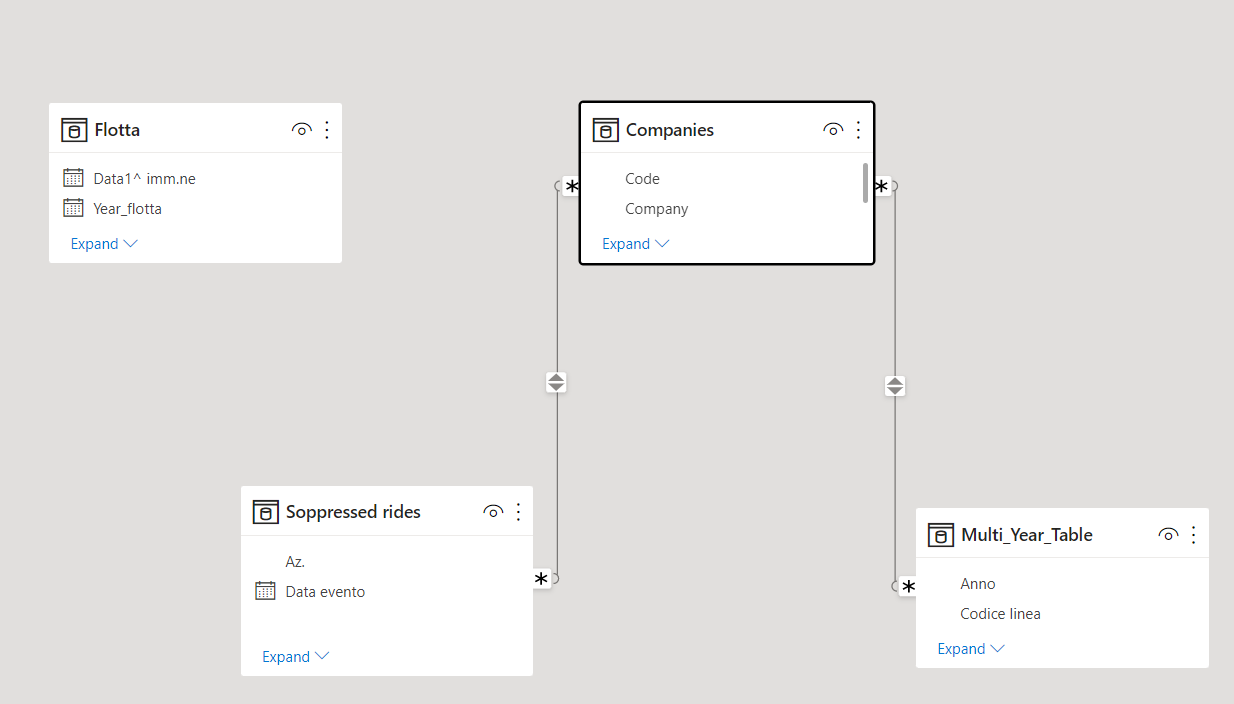
\includegraphics[width=0.9\textwidth]{Images/traditional_dashboard/ER_model.png}
    \caption{ER model of the Dashboard}
    \label{fig:ER}
\end{figure}
\section{Dashboard}

Starting from these tables, a dashboard is designed. It will be divided in subcategories that differ each other for the topic shown. In particular, the themes approached are:
\begin{itemize}
\item Suppressed rides
\item Emissions
\item Operative performances
\item KPIs correlation
\item Economics
\end{itemize}
\subsection{Suppressed rides}
In the following page has been presented the dashboard
\newpage
\begin{landscape}
\thispagestyle{empty}
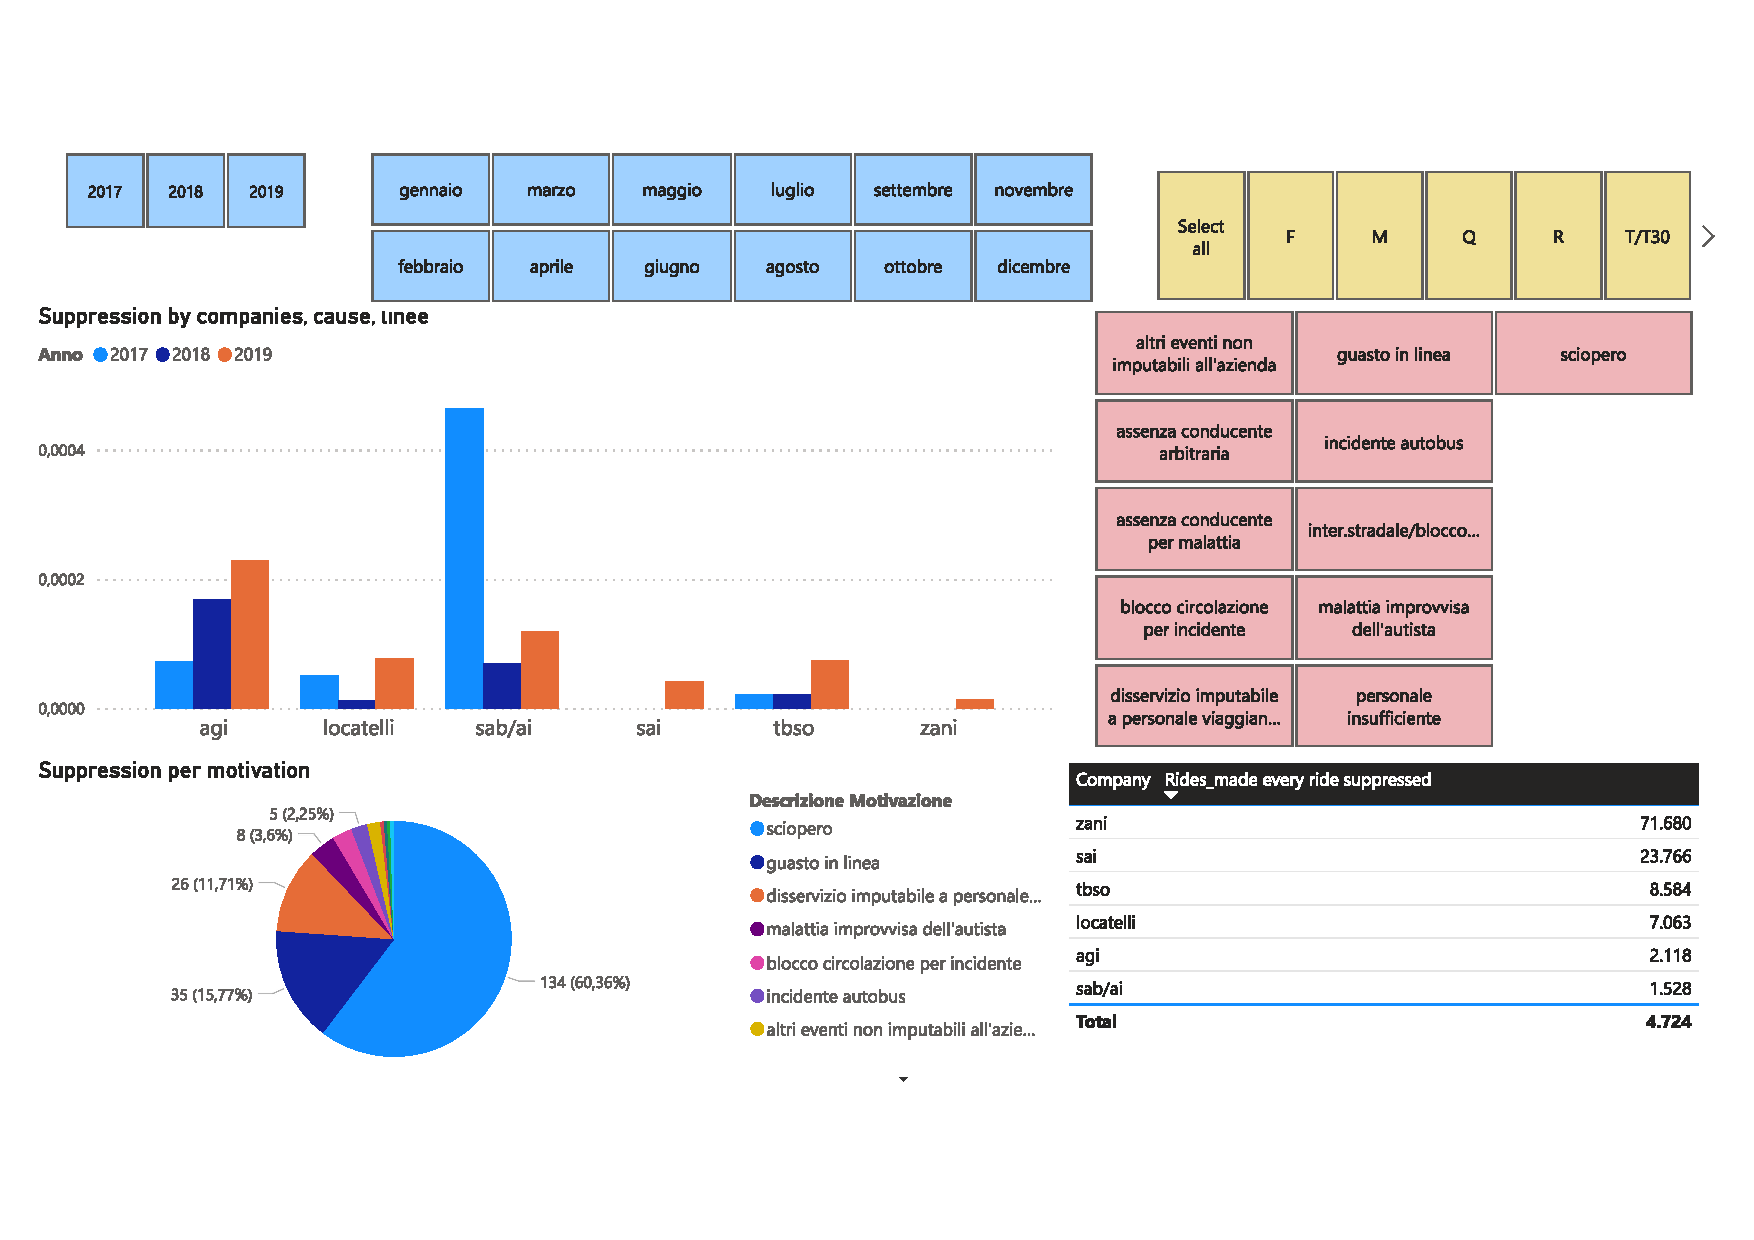
\includepdf[angle=90, pagecommand={\null\enlargethispage{2\baselineskip}\vfill\captionof{figure}{Suppressed}}]{dashboard/Suppression.pdf}
\end{landscape}
\newpage
As said before, data about suppressed rides are between 2017 and 2019. An area of this part of the page is dedicated to filters, thanks to which data can be visualized according to:
\begin{itemize}
\item  period of time with a level of detail equal to a month
\item line
\item reason for which the ride was suppressed
\end{itemize}
Obviously, these filters could be used at the same time in order to obtain very specific analysis.

The table on the bottom right shows the number of rides traveled per each ride suppressed for each company. So, a low number corresponds to a bad result for the company. This data is computed in a relative way in order to show if a company has bad performances according to its dimension. A ride suppressed for a small company is not comparable with few rides suppressed for a big one. 

The pie chart has the goal of showing how the different causes affects suppressed rides, while the histogram shows the total suppressed rides for each year divided by company. 

Considering the dashboard without applying any filter, some considerations can be already done. In 2017 Sab/ai had a huge issue with suppressed rides that reached a percentage level double than the second highest one, in the analyzed period. In 2017 and 2018 Sai and Zani had no problems and their suppressed rides are equal to zero. Finally, Agi had a ever increasing problem related to suppressed rides. 

Moreover, the main cause that brings to a suppressed ride is strike followed at a distance by failure happened during service and inconvenience due to drivers during service. 

Finally, companies with performances below Consortium average are Agi and Sab/ai with, respectively, a ride suppressed every 2,118 and 1,528 rides traveled. 

\newpage

\begin{landscape}
\thispagestyle{empty}
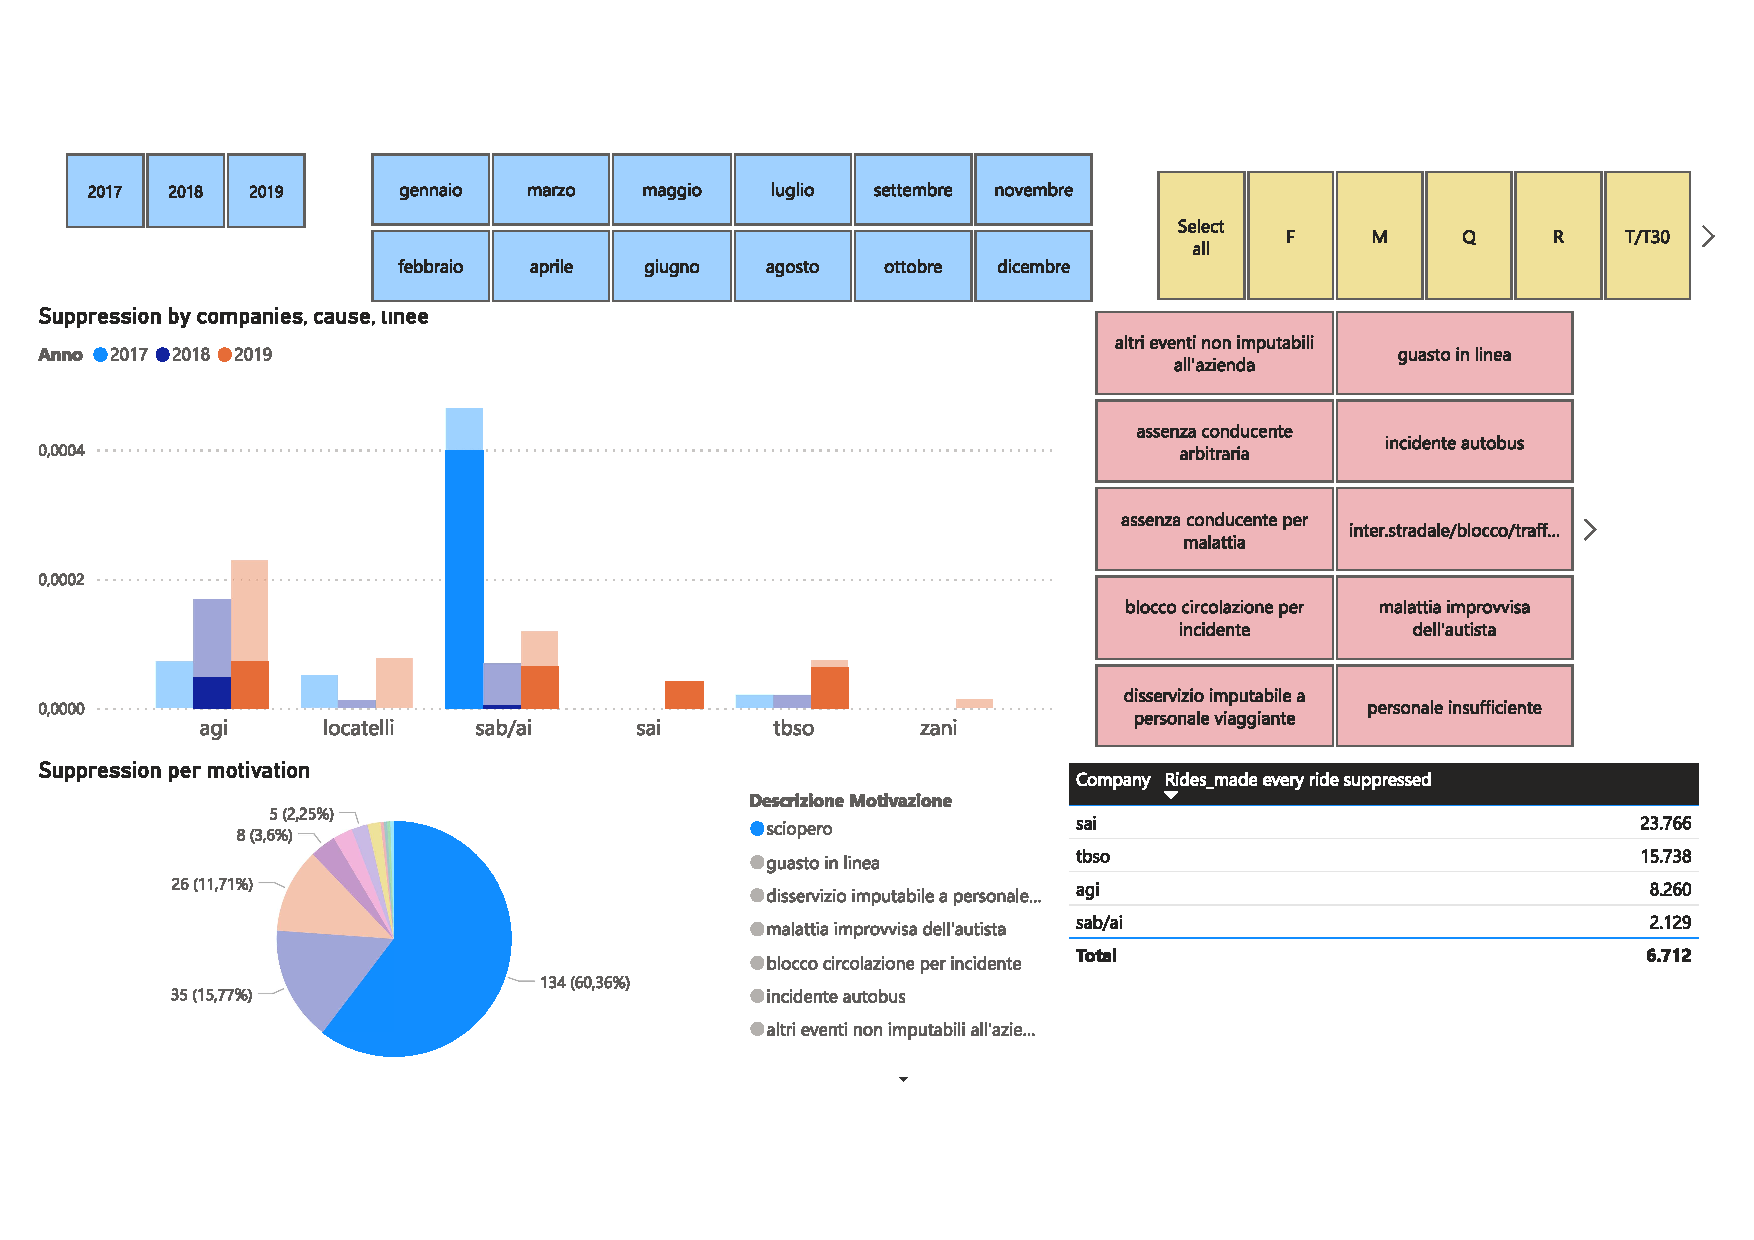
\includepdf[angle=90,  pagecommand={\null\enlargethispage{2\baselineskip}\vfill\captionof{figure}{Suppressed for strikes}\label{fig:strikes}}]{dashboard/Suppression_for_strikes.pdf}
\end{landscape}
\newpage

A focus on the strikes, shown in figure \ref{fig:strikes}, gives several information. Strikes are the reason of the abnormal problems tha Sab/ai had in 2017, moreover a strike in 2019 hit almost every company in an equal measure and, finally, Agi growing issues during this period are reflected also in strikes trend. 

Filtering data according to failure happened during service, a very interesting result is shown: half of the total failures happened during the three year in the Consortium happened during a ride performed by Agi even if Agi is one of the companies with less kilometers run per year. Moreover, this problem in absolute terms remains constant during the year and the negative trend of Agi is due to the increasing of other issues that in 2017 were almost absent.

\newpage
\begin{landscape}
\thispagestyle{empty}
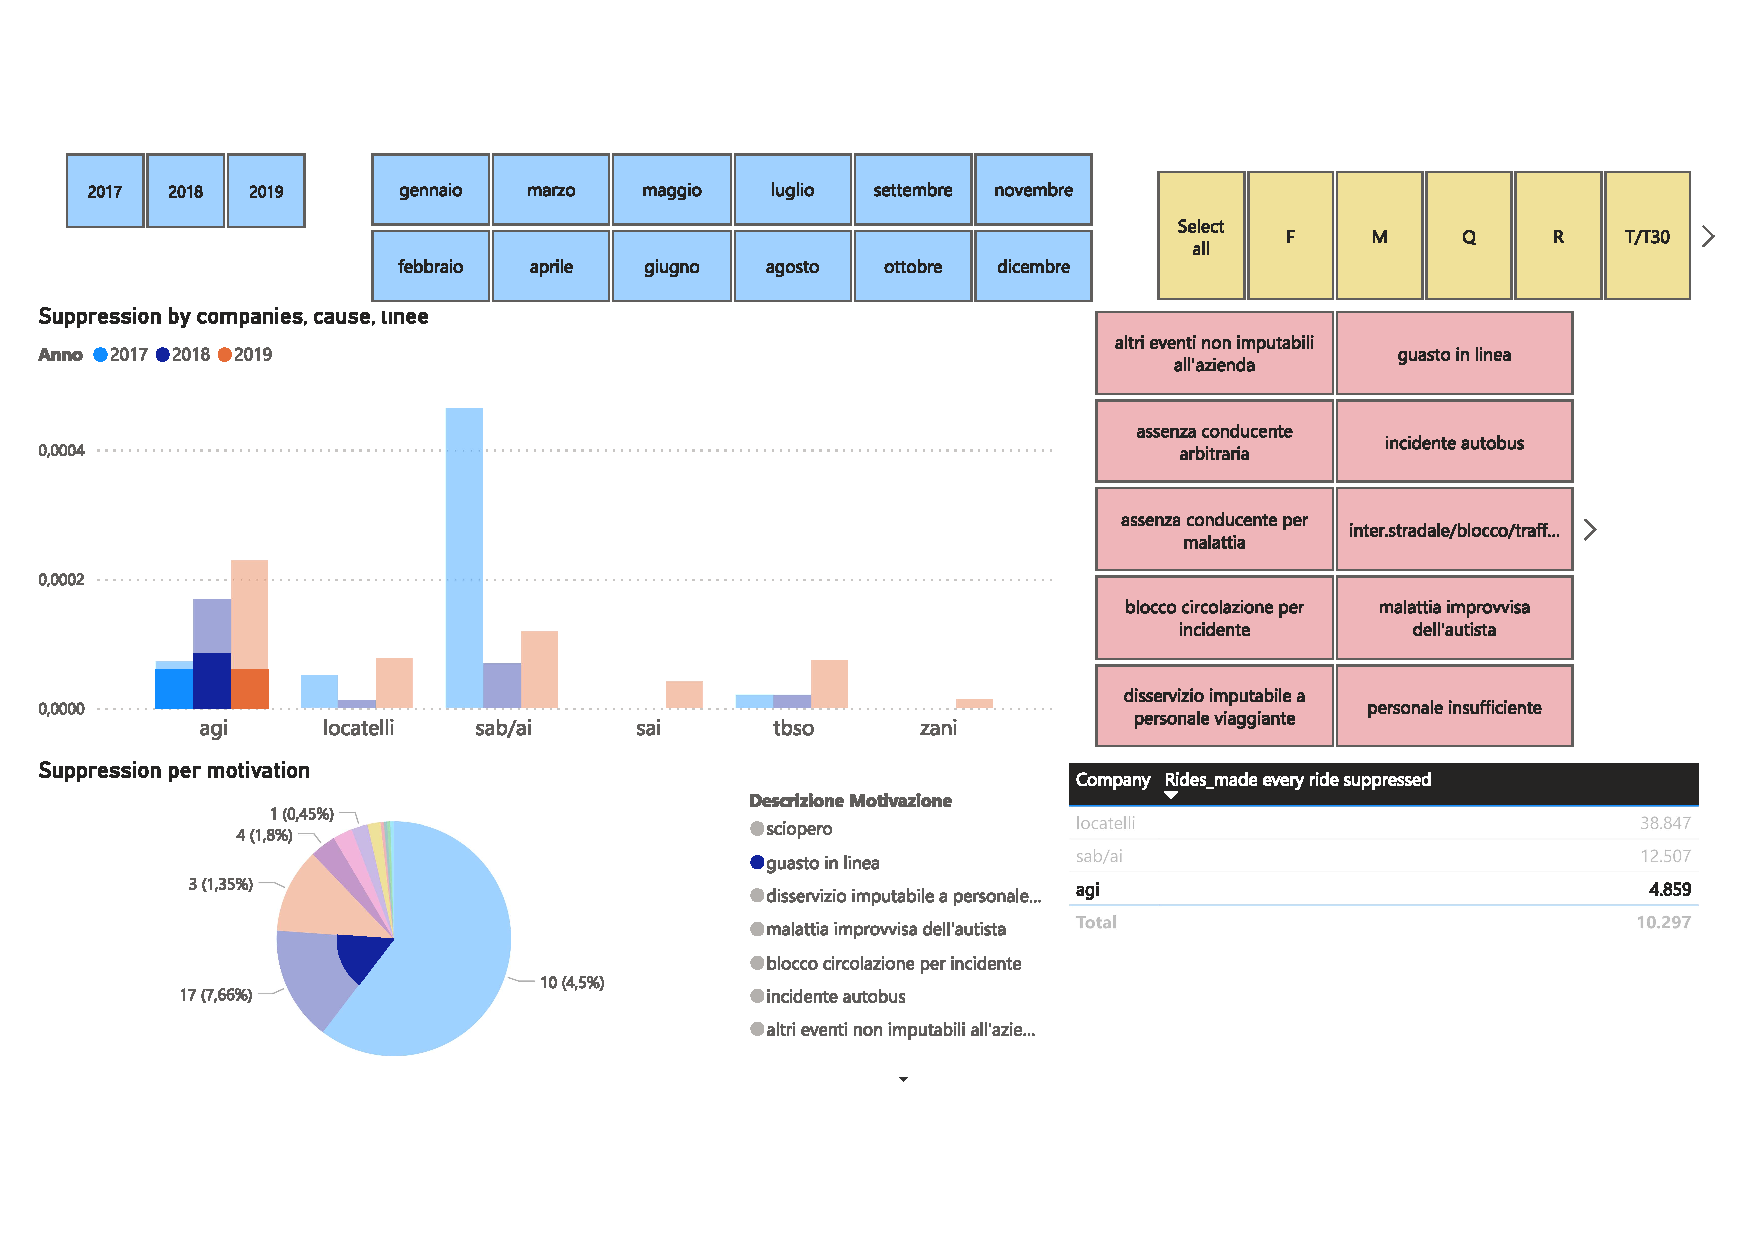
\includepdf[angle=90, pagecommand={\null\enlargethispage{2\baselineskip}\vfill\captionof{figure}{Focus on Agi and fault on the line}\label{fig:failline}}]{dashboard/Suppression_for_fail_on_the_line.pdf}
\end{landscape}
\newpage

\chapter{Innovative KPI}

From sustainability balance sheets
From new technologies installed on buses now and in the next future



%-------------------------------------------------------------------------
%	BIBLIOGRAPHY
%-------------------------------------------------------------------------

\addtocontents{toc}{\vspace{2em}} % Add a gap in the Contents, for aesthetics
\bibliography{Thesis_bibliography} % The references information are stored in the file named "Thesis_bibliography.bib"

%-------------------------------------------------------------------------
%	APPENDICES
%-------------------------------------------------------------------------

\cleardoublepage
\addtocontents{toc}{\vspace{2em}} % Add a gap in the Contents, for aesthetics
\appendix
\chapter{Appendix A}
If you need to include an appendix to support the research in your thesis, you can place it at the end of the manuscript.
An appendix contains supplementary material (figures, tables, data, codes, mathematical proofs, surveys, \dots)
which supplement the main results contained in the previous chapters.

\chapter{Appendix B}
It may be necessary to include another appendix to better organize the presentation of supplementary material.


% LIST OF FIGURES
\listoffigures

% LIST OF TABLES
\listoftables

% LIST OF SYMBOLS
% Write out the List of Symbols in this page
\chapter*{List of Symbols} % You have to include a chapter for your list of symbols (
\begin{table}[H]
    \centering
    \begin{tabular}{lll}
        \textbf{Variable} & \textbf{Description} & \textbf{SI unit} \\\hline\\[-9px]
        $\bm{u}$ & solid displacement & m \\[2px]
        $\bm{u}_f$ & fluid displacement & m \\[2px]
    \end{tabular}
\end{table}

% ACKNOWLEDGEMENTS
\chapter*{Acknowledgements}
Here you might want to acknowledge someone.

\cleardoublepage

\end{document}
